\chapter{Programming Language Verification }
\graphicspath{ {./images/} }

Any computer programming language consists of type system to its core supported by data structures and control flow techniques. Any Programming language finally can be broken down to machine codes resulting in perfoming specified actions. The assembly level machine codes should theoretically represent the same semantics as implied by the higher order programming language. \textbf{Programming Language Verification} in the broader sense is checking that programs in one programming language is equivalent to the one in other. Generally this equaivalence is tested between a high order	language and a small low level C language. \\

The basic understanding of how the verification work can be thought as, say there are two programs e$_1$ and e$_2$ then to prove they are equivalent the must meet the following criteria :

\begin{itemize}

\item{
	Input Parameters as well as the context in which the program is being run is same. Input parameters can be thougt as some initial values to a program. Input parameters should necessarily be of same type. The context refers to same harware used as well as the scope of the program in consideration is maintained same. Context can then again be broken as a \textit{Global} context and a \textit{Local} context. 
}

\item{
	The result should be same and should be of the same type. It is necessary that any program should not violate any of the bonding rules imposed by context.
}

\end{itemize}    

How do we check this ?\\

Well the method used is called \textbf{Step-Indexing}\cite{step_indexing}. In this method we look for holes in a program. These holes represented by C$_i$ can be thought as a program's loop structure or the way conditional arguments have been put up. In any step of a program thus if we are able to show that at that point, C$_2$[e$_1$] termminates and C$_1$[e$_2$] termminates also producing same results then we have shown the programs are equal. The cardinality issues related to number of such possible holes in programs increases the complexity of verification proof. This method therefore says that we should unfold the program upto required N steps and consider the equivalence then.\\

The areas where this method stucks is where we are unable to predict N. This is the case of IO type functions. The work on this is going on and improved proofs are being generated.\\


\section{Verified Software Toolchain}
This project \cite{VST} led by Princeton University deals with verifying software programs and compilers. It is an advancement to Compcert. It uses multi layered kernels to securely verify the programs.  

\begin{figure}[!htb]
\centering
  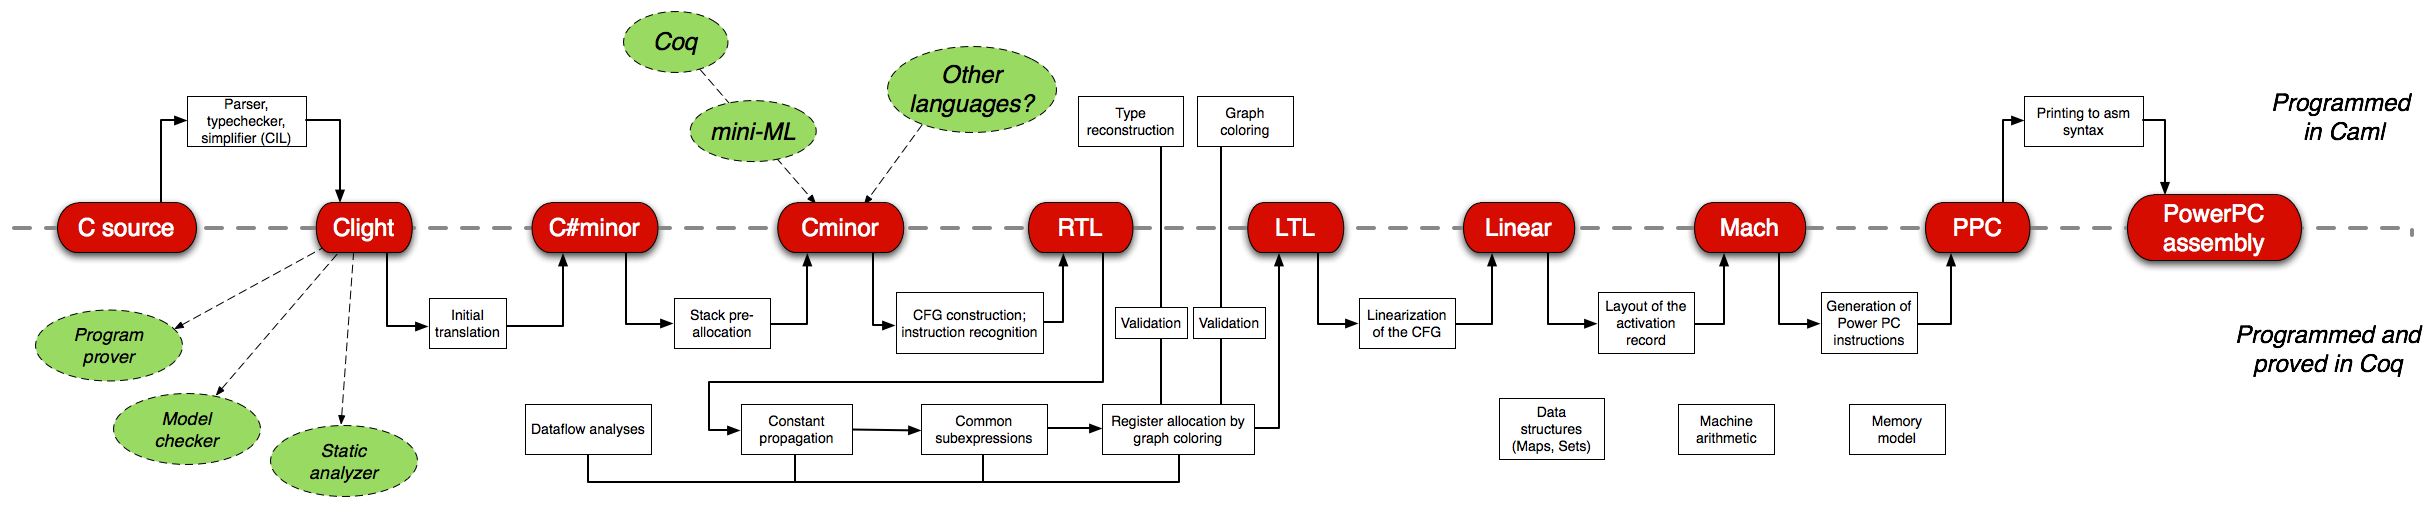
\includegraphics[width=\textwidth]{diagram}
  \caption{Flow diagram of CompCert C ( Source: Official Site)}
\end{figure}

The software toolchain includes static analyzers to check assertions about programs; optimizing compilers to translate programs to machine language operating systems and libraries to supply context for programs. Verified Software Toolchain verifies with machine-checked proofs that the assertions claimed at the top of the toolchain really hold in the machine-language program, running in the operating-system context, on a weakly-consistent-shared-memory ma-
chine.


